\documentclass[12pt,fleqn]{article}\usepackage{../../common}
\begin{document}
Türevler

Türev İşlevi Nasıl Türetilir

Calculus, bir veya daha fazla dereceli denklemlerin, en yüksek noktasını
bulmak, değişimi temsil etmek gibi birçok bilim ve mühendislik alanında
kullanılır. Herhalde Calculus'in türev, entegral alma gibi yöntemlerini
şimdiye kadar çok gördük. Fakat genelde anlatılmayan, türev ve entegral
işlemlerinin nasıl yapıldığı, yani Calculus'in nasıl işlediği.

Örnek olarak, aşağıdaki grafiğe bakalım. 

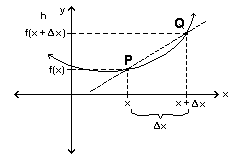
\includegraphics[height=4cm]{calc_multi_app_10.png}

Gösterilen eğri, $x^2$ eğrisi. Bu eğrinin artış oranını bulmak için, artış
oranını temsil eden işlevi bulabiliriz. Bu işleve türev alarak gideceğiz.

Bunu yapmanın bir yolu, y eksenindeki artışı x eksenindeki artış ile
bölmek. 

$$ f(x) = x^2 $$

$f(x)$'in türevini bulmak için 

$$ = \frac{f(x+\Delta x) - f(x)}{\Delta x} $$

$$ = \frac{(x+\Delta x)^2 - x^2}{\Delta x} $$

$$ = \frac{x^2 + 2x\Delta x + \Delta x^2 - x^2}{\Delta x} $$

$x^2$'ler iptal oldu

$$=  \frac{2x\Delta x + \Delta x^2}{\Delta x} $$


$$ = 2x + \Delta x $$

Bu elimizdeki işlev, türevin son haline yaklaştı. En son haline getirmek
için, şöyle düşünmemiz gerekiyor. Artış miktarını bulduk, ama x eksenindeki
artış basamağı ne kadar büyük olmalı? Sonuna kadar küçültürsek, elimize
hangi işlev geçer?

Calculus'u ilk bulan Leibniz adlı matematikçi, zamanına göre büyük bir
ilerleme olan bu yeni metodu bir türlü meslektaşlarına tarif
edemiyordu. "$x^2$'nin türevi nasıl 2x oluyor" gibi sorulara, artış miktarı
kavramını anlatıyor, fakat $2x$ formülüne geldiğini bahsederken, "$x$'teki
artış sonsuz küçüldüğü için $2x$'e yaklaşıyoruz" deyince, arkadaşları onu
anlamıyordu. Zamanın matematikçileri bu 'sonsuz küçüklük' kavramını çok
eleştirdiler. Leibniz sonunda, "sonsuz küçük sayıların olduğu delilik gibi
gelebilir, fakat pratik hesaplamalar açısından yararlı bir alet olarak
Calculus'un hala yararlı olabileceğini düşünüyorum" demişti. Yani
Calculus'un matematiksel ispatı Leibniz zamanında yapılamadı. Keşifler
tarihin de bu olağan bir durumdur. Türevler, zamanı için yeterince normal
dışı bir buluştu, bunun üzerine hemen arkasından bir diğer sarsıcı buluşun
yapılması, çoğu zaman mümkün olmamaktadır.

Bu yüzden türevlerin soyut matematiksel olarak ispatının yapılması, 1821'de
limit kuramının keşfine kadar beklemiştir. Fakat bu keşiften önce bile,
mühendisler ve bilim adamları Calculus yöntemlerini verimli bir şekilde
kullanmaya başlamışlardı.

Sonsuz Küçüklük

Leipniz ve Calculus'un ``öteki babası'' sayılan Newton'un söylemeye
çalıştıkları, türev işleminin bir durağan resim üzerinde yapılan hesap
değil, ardışıl yaklaşıklama süreci altında bir sabit sonuca "yaklaşan"
hareketli bir hedef olduğu idi. Matematiksel limit kuramı, bu tür bir
tarifi gösterebildiği için sonunda Calculus'u ispatlamak mümkün oldu.

$$ g(x) = 2x + \Delta x $$

$$ \lim_{\Delta x \to 0}g(x) = \lim_{\Delta x \to 0} (2x + \Delta x)  $$

$$ \lim_{\Delta x \to 0}g(x) = 2x$$

Bu formüle bakarak bir daha belirtmek gerekir ki, $x$ değişimini 0'a
eşitlemiyoruz. 0'a eşitleseydik, daha baştan bölünen olarak elimize sıfır
geçeceği için cebirsel işlemde bu kadar ilerlememiz mümkün
olmazdı. Yaptığımız, limit tarifini kullanarak, $x$ sıfıra yaklaşırken
türev $2x$'e yaklaşır demektir.

Bu tanım sonucu elde ettiğimiz yeni fonksiyon da, tüm diğer fonksiyonlar
gibi, aynen limitlerin çalıştığı uzayda olduğu gibi sonsuz küçük
aralıklarla çalışabilecek bir tanım olduğu için, bu türetilmiş yeni
fonksiyonu da normal bir fonksiyon olarak kabul etmemiz mümkün olmaktadır.

Türev: $\sin(x)$

[1, sf. 66]. Sinüs fonksiyonunun türevi derken aslında kastedilen şudur,

$$ \lim_{h \to 0} \frac{sin(x+h) - sin(x)}{h} $$

Trigonometrik eşitliklerden bildiğimize göre, 

$$ sin(a+b) = \sin a \cos b + \cos a \sin b $$

Bu eşitliği iki üstteki fonksiyonu açmak için kullanalım,

$$ \lim_{h \to 0} \frac{\sin x \cos h + \cos x \sin h - \sin x }{h} $$

$$ = \lim_{h \to 0} \sin x \bigg( \frac{\cos h - 1}{h} \bigg) + \cos x \bigg( \frac{\sin h}{h} \bigg) $$

Pür trigonometri ve cebir bizi buraya getirdi; bundan sonrası limitler ve
Calculus. Şu soruyu soralım, $h \to 0$ iken üstteki formüllere ne olur? 

Limit: $\sin h / h$

Önce $\sin h / h$'e bakalım. Ufak $h$ değerleri için 

$$ \sin h < h, \qquad \tan h > h $$

eşitsizliklerinin doğru olduğunu biliyoruz. Ya da

$$ \frac{\sin h}{h} < 1, \qquad  \frac{\sin h}{\cos h} > h $$

İkinci eşitsizliği biraz değiştirelim,

$$ \frac{\sin h}{h} < 1, \qquad  \frac{\sin h}{h} > \cos h $$

Şimdi bu eşitsizlikleri ispatlayalım. 1. eşitsizliğin ispatı için alttaki
figür yeterli,

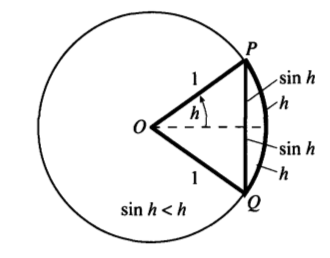
\includegraphics[height=4cm]{calc_multi_app_01.png}

İki nokta arasındaki en kısa mesafe düz çizgi olduğuna göre $2h < 2\sin h$
olmalı, yani $\sin h < h$, ya da $\sin h / h < 1$.

2. eşitsizliğin ispatı için alan hesabını kullanacağız. 

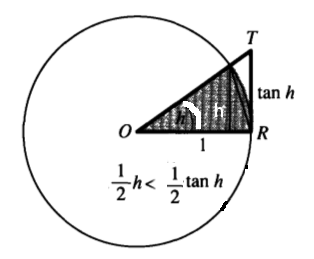
\includegraphics[height=4cm]{calc_multi_app_02.png}

Üstteki figürdeki üçgenin alanı $\tan h \cdot 1 / 2$'dir, değil mi, çünkü
üçgen alanı iki kenarın çarpımının iki ile bölümüne eşittir, kenarın
büyüklüğü $\tan h$, bunu temel trigonometriden biliyoruz, diğer kenar ise
1. Gri alan ise dairenin bir parçası, onun $h/2\pi$'lik oranında bir
parçası daha doğrusu, ve o parçanın alanı alanı $h/2\pi \cdot \pi r^2$,
$\pi r^2$ tüm alanı temsil eder, $r=1$ olduğuna göre sonuç $1/2 h$. Eh,
dairenin parçası olan alan onu kapsayan üçgenden daha küçük olduğuna göre
$1/2 h < 1/2 \tan h$, yani $h < \tan h$. İspat tamam.

Şimdi $h \to 0$ iken ne olur? Formüllere tekrar bakalım,

$$ \frac{\sin h}{h} < 1, \qquad  \frac{\sin h}{h} > \cos h $$

Bu durumda $\cos h$ zaten 1'e yaklaşıyordu (çünkü $\cos 0 = 1$), yani $\sin h
/ h$ hem 1'den küçük olmak hem de 1' yaklaşmak arasında ``sıkışacak
(squeezed)''. O zaman limite giderken bu değer 1'e yaklaşmalıdır.

Limit: $(\cos h -1) / h$ Sıfıra Gider

Bu ispat için $(\sin h)^2 + (\cos h)^2 = 1$'den faydalanacağız. 

$\sin h < h$ olduğunu artık biliyoruz, onu üstteki formüle koyalım,

$$ (\sin h)^2 = 1 -  (\cos h)^2$$

$$ h^2 > 1 -  (\cos h)^2$$

Üstteki ifadelerin hepsinin pozitif olduğuna dikkat, çünkü $h^2$ bir kare
işlemi, ayrıca $\cos h$ $h$ sıfıra ``yaklaşırken'' 1'e yaklaşır, o zaman
$1-\cos h$ her zaman sıfırdan büyük olur. Bunu ekleyelim, bir de ufak
açılım yapalım,

$$ 0 > h^2 > (1 + \cos h)(1 - \cos h)$$

Şimdi tüm terimleri önce $h$ sonra $1+\cos h$ ile bölersek, 

$$ 0 < \frac{1 + \cos h}{h} <  \frac{h}{1+\cos h} $$

Yine arada sıkışmışlık argümanını kullanacağız, $h \to 0$ iken en sağdaki
formül sıfıra gider, ve ortadaki formül 0 ile 0'a gitmek arasında
sıkışır. Demek ki ortadaki ifade de sıfıra gider.

Şimdi ana ifadeye dönelim. $h$ sıfıra giderken $\sin h/h$ 1'e gidiyor,
$(\cos h-1)/h$ ise sıfıra gidiyor, o zaman üstteki formülde geriye tek
kalan $\cos x$ ifadesidir. 

$$ \lim_{h \to 0}  
\sin x \bigg( \cancelto{0}{\frac{\cos h - 1}{h}} \bigg) + 
\cos x \bigg( \cancelto{1}{\frac{\sin h}{h}} \bigg)
$$

$$ = cos(x) $$

Böylece $\sin x$'in türevinin $\cos x$ olduğunu ispatlamış olduk.

Dolaylı Türev Almak (Implicit Differentiation)

Türev alırken başlangıçta $y = x^2$ turu $y$'yi direk $x$ ile ilintilendiren
açık, belirtilmiş, belli (explicit) fonksiyon varlığı farz edilir. Fakat bazen
elde dolaylı $x^2+y^2 = 9$ gibi bir fonksiyon olabilir burada her iki değişken
arasında bir alaka vardır fakat bağımlı, bağımsız değişken yoktur, gösterilen
ilişkiyi tatmin eden tüm $x,y$ değerleri geçerli değerlerdir. 

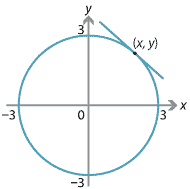
\includegraphics[width=20em]{calc_multi_app_03.png}

Fakat bu durumda herhangi bir $x,y$ noktasındaki eğriye teğet çizgiyi nasıl
buluruz? Dolaylı türev alarak bunu başarabiliriz [2], yine $\frac{\ud}{\ud x}$
türevini alıyoruz ve uzun uzadıya $y$'yi $x$ üzerinden bir sürü cebirsel takla
ile temsil etmeye uğraşmadan türev işlemi bu alakayı farz ediyor, ve gerektiği
yerde Zincirleme Kuralı kullanıyor.

$$
\frac{\ud}{\ud x} (x^2)  + \frac{\ud}{\ud x} (y^2) = \frac{\ud}{\ud x} (9)
$$

İlk terim basit, $2x$. İkinci terimde Zincirleme Kuralı lazım,

$$
\frac{\ud}{\ud x} (y^2) = \frac{\ud}{\ud x} (y^2) \frac{\ud y}{\ud x} =
2y \frac{\ud y}{\ud x}
$$

Üçüncü terim sabitin türevi olduğu için sıfır. Yani

$$
2x + 2y \frac{\ud y}{\ud x} = 0
$$

Şimdi $\ud y / \ud x$ için düzenleme yaparsak,

$$
\frac{\ud y}{\ud x} = -\frac{x}{y}
$$

elde ederiz. 

Kaynaklar

[1] Strang, {\em Calculus}

[2] AMSI, {\em Implicit differentiation},
    \url{https://www.math.ucdavis.edu/~kouba/CalcOneDIRECTORY/implicitdiffdirectory/ImplicitDiff.html}

\end{document}
